\section{Introduction}

%vis centric overview...
%Adios makes use of an operation that is already being done by data producers and data consumers: reading and writing files. 
%Adios serves as a middleware layer between applications and the computing system.  From the perspective of a data producer, the application is writing data using a file like abstraction. From a data consumer, it is also reading data from a file like abstraction.
%adios makes use of what a data producer is already doing: writing data.

The Adaptable I/O System (ADIOS) was designed with the observation that applications almost universally read and write files from storage, and that this can be used as an abstraction for access to data~\cite{godoy2020}. ADIOS is a middleware layer that sits between the application and the computing system to manage the movement of data. This middleware layer makes it possible for an application to write data to a target that is determined at runtime. One possible target is traditional file storage. 
Other targets are able to support in situ processing methods, and include a memory buffer on the nodes where the application is running, or over the network to a memory buffer on another set of resources. Applications (e.g., visualization and analysis codes) can read data from any of the file or in situ targets. A schematic showing examples of these use cases in given in Figure~\ref{ch10:fig:adios_design}.  The advantage of this design is that the sharing and movement of data is decoupled from the producer and the consumer, and can be modified at runtime as needed. This advantage addresses several of the challenges described in Section~\ref{intro:challenges} of Chapter~\ref{chapter:intro}. Workflow execution is made easier when data producers and consumers can be connected together without modifying the source codes. Software complexity is reduced because the issues related to data access across evolving systems are provided by the middleware layer. Better resilience is possible because the producer and consumer need not run together in the same memory space.

\begin{figure}[htb]
    \centering
    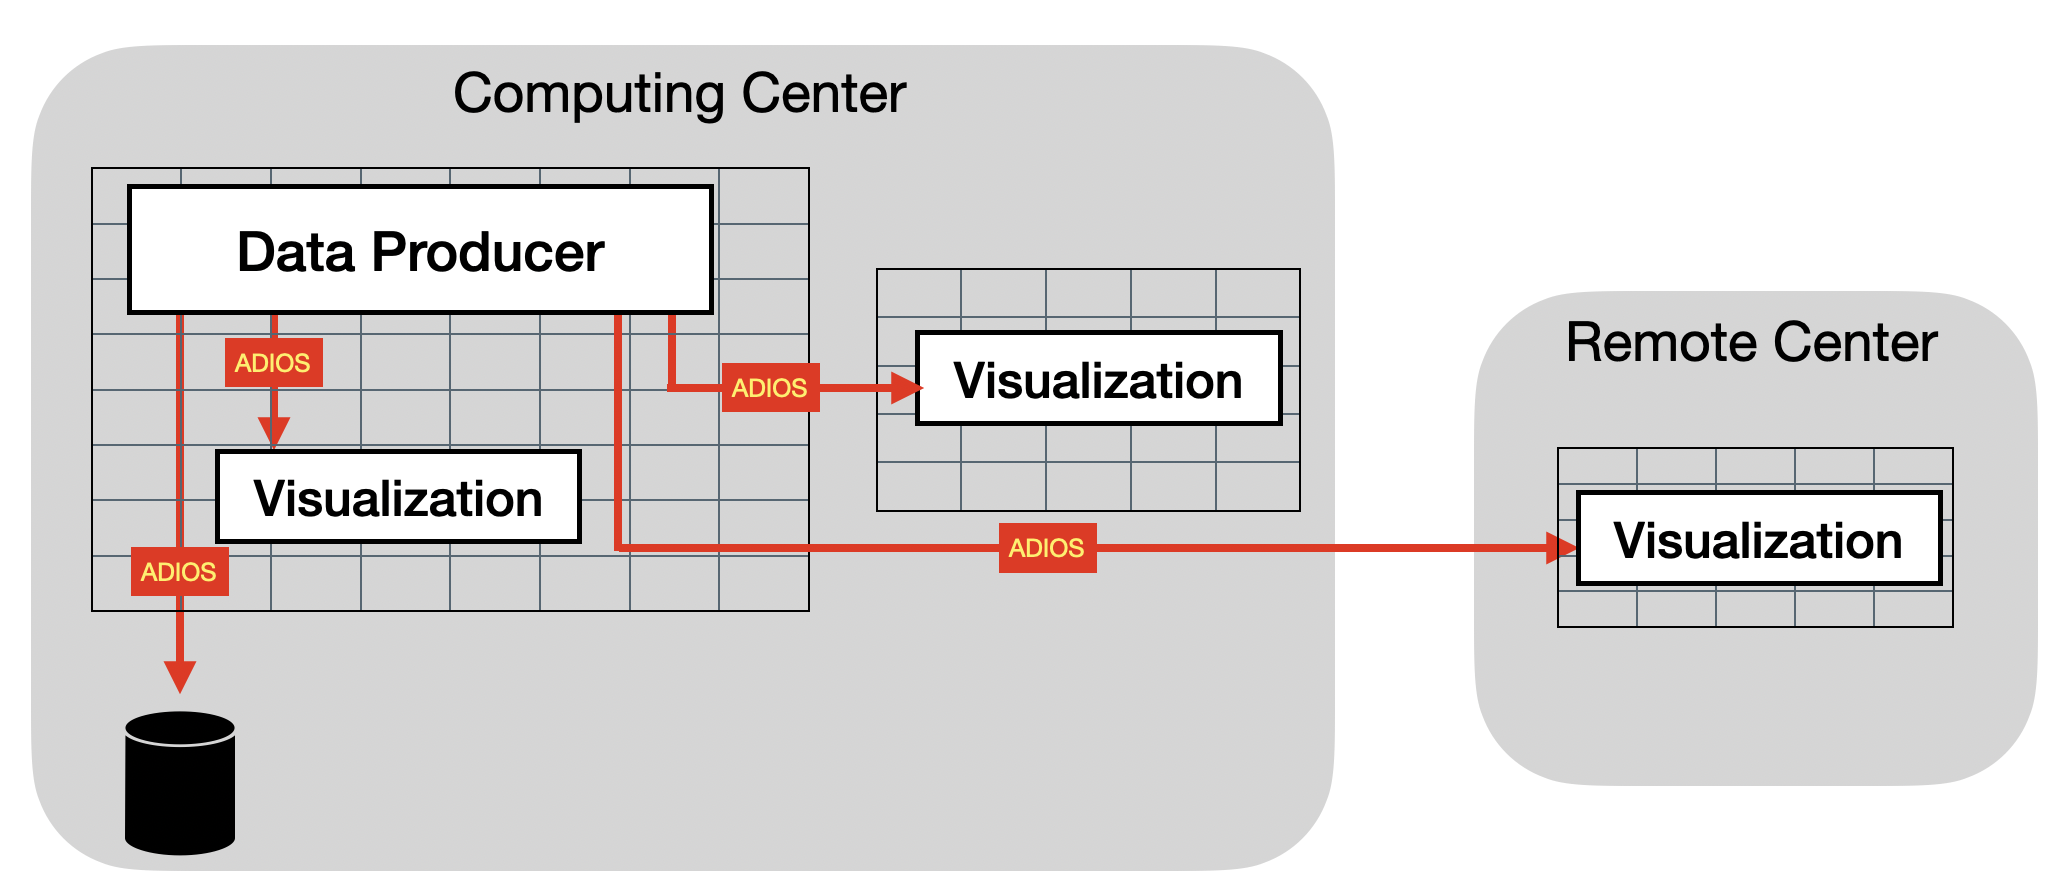
\includegraphics[width=4in]{figures/ADIOS}
    \caption{Examples of ADIOS usage. In this example, the producer can write data to disk, to a visualization process sharing the same resource as the simulation, to a separate set of nodes, or across the network to a remote computing center.}
    \label{ch10:fig:adios_design}
\end{figure}


In terms of the taxonomy described in Section~\ref{intro:taxonomy} of Chapter~\ref{chapter:intro}, ADIOS can be classified in the following ways. \emph{Integration type}: Apart from the usage of the ADIOS API for I/O, no additional instrumentation is needed by the application. \emph{Proximity}: The visualization can run on the same or different computing resources. \emph{Access}: The visualization can directly access memory in the simulation, or it can be copied to a memory buffer on the same or on different computing resources. \emph{Division of Execution}: Synchronous or asynchronous are both possible, providing support for both time and space division.  \emph{Operation Controls}: Human in the loop is possible using both synchronous (blocking) or asynchronous (non-blocking) modes.


The ADIOS framework design was based on the goal to provide an I/O abstraction for parallel and distributed applications that expresses \emph{what} data is produced for output and \emph{when} that data is ready for output, or what data an application wants to read and when\cite{liu2014hello, Logan2020, osti_1468120}.
This is achieved in ADIOS through the use of different types of I/O \emph{engines}. When an application writes a set of data, it uses the appropriate engine (e.g., File engine, In situ engine, etc) to do the actual data movement. Similarly for a reader, it uses the appropriate Engine to request the data that it needs. For flexibility, the types of engine used by producer and consumer can be specified in a configuration file for runtime selection.
In this way, applications that either read or write data need only select the appropriate output engine, and do not need to be concerned with the implementation details needed to achieve scalable performance.


%ADIOS was designed with the observation that, from an application point of view, there is not much difference between writing and reading data from storage and coupling independent application codes together.
%The main goal of the ADIOS framework design is to provide an I/O abstraction for parallel and distributed applications, that expresses \emph{what} data is produced for output and \emph{when} that data is ready for output, or what data an application wants to read and when.
%Crucially, the concept of permanent storage or a connected application, i.e., the target of the output or the source of the input, is omitted from the abstraction.
%The I/O \emph{strategy} is dependent on what the input sources and output targets are, and is implemented by a designated ADIOS \emph{Engine}.
%Therefore, an application can use ADIOS to produce an output data stream without concerning itself with where the data goes, and then choose the proper engine at runtime to store data on disk or to stream it to a consumer application. 

The separation of concerns, namely that an application only need to be concerned about the data production and consumption but not how the data should be delivered, allows for creating optimized ADIOS engines that all can work with the same application code.
Using the ADIOS interface makes application I/O \emph{scalable}, a primary goal of the ADIOS framework, which is designed to work well on the largest supercomputers. ADIOS regularly runs on the largest supercomputers in the world for applications that consume and produce multiple petabytes of data during the course of a simulation run.

%There are applications, like Specfem3d\_globe\cite{specfem3d}, PIConGPU\cite{picongpu} and XGC\cite{xgc}, that regularly produce and consume petabytes of data on the leadership computing facilities around the world using ADIOS for storage I/O. 

In this chapter we describe details of the ADIOS framework and how it can be used for in situ visualization. In Section~\ref{sec:adios} we describe the I/O abstractions used by ADIOS and how applications and visualization codes can use them. Section~\ref{sec:adios:engine} provides a description of the engines provided by ADIOS and how they handle the movement of data. Advanced features in ADIOS are described in Section~\ref{sec:adios:advanced}, followed by a  discussion on the relative strengths of each engine and coding examples in Sections~\ref{sec:adios:discussion} and~\ref{sec:adios:code}. In Section~\ref{sec:examples} we describe the use of ADIOS for in situ visualization with application partners, followed by some concluding remarks in Section~\ref{sec:conclusion}.

%In this chapter, we focus on other capabilities borne from this I/O abstraction. Since the application output code only defines what the output data is and when it is ready for output but does not encode anything about how the output is performed, the output data can move to different targets depending on the engine that connects the application to the target. It can be used for strong coupling of simulation codes, for in situ visualization running on a separate computing cluster, and for streaming experimental data between Asia and the United States.

